% This LaTeX was auto-generated from MATLAB code.
% To make changes, update the MATLAB code and export to LaTeX again.

\documentclass{article}

\usepackage[utf8]{inputenc}
\usepackage[T1]{fontenc}
\usepackage{lmodern}
\usepackage{graphicx}
\usepackage{color}
\usepackage{listings}
\usepackage{hyperref}
\usepackage{amsmath}
\usepackage{amsfonts}
\usepackage{epstopdf}
\usepackage[table]{xcolor}
\usepackage{matlab}

\sloppy
\epstopdfsetup{outdir=./}
\graphicspath{ {./indirect_methods_images/} }

\begin{document}

\label{H_F0E5F1DD}
\matlabheading{Computational Methods in Ordinary Differential Equations}

\begin{par}
\begin{flushleft}
\textit{Dr Jon Shiach, Department of Computing and Mathematics, Manchester Metropolitan University}
\end{flushleft}
\end{par}

\label{T_C94928D2}
\matlabtitle{Indirect Methods for Solving Systems of Linear Equations}


\vspace{1em}
\begin{par}
\begin{flushleft}
\textbf{Learning outcomes}
\end{flushleft}
\end{par}

\begin{par}
\begin{flushleft}
On successful completion of this page readers will be able to:
\end{flushleft}
\end{par}

\begin{itemize}
\setlength{\itemsep}{-1ex}
   \item{\begin{flushleft} Understand the concept of an \hyperref{H_52186026}{indirect method} when used to solve a system of linear equations. \end{flushleft}}
   \item{\begin{flushleft} Apply the \hyperref{H_55926E44}{Jacobi}, \hyperref{H_CAC75FFA}{Gauss-Seidel} and \hyperref{H_0296912E}{SOR} methods to solve a linear system. \end{flushleft}}
   \item{\begin{flushleft} Use the \hyperref{H_F86E4C8E}{residual} to determine the accuracy of the current estimate of the solution to the linear system. \end{flushleft}}
   \item{\begin{flushleft} Determine whether an indirect method is \hyperref{H_0FAA1538}{convergent} for a particular linear system and anaylse the theoretical rate of convergence for indirect methods. \end{flushleft}}
\end{itemize}


\vspace{1em}
\label{H_52186026}
\matlabheading{Indirect Methods}

\begin{par}
\begin{flushleft}
Indirect methods for solving systems of linear equations use an iterative approach to repeatedly update estimates of the exact solution to the linear system. They are called \textit{indirect} methods since multiple applications of the method is required to calculate a solution unlike \textit{direct} methods such as \href{https://en.wikipedia.org/wiki/Gaussian_elimination}{Gaussian elimiation} and \href{https://en.wikipedia.org/wiki/LU_decomposition}{LU decomposition} which require a single application to calculate the solution. However, direct methods are inefficient for large systems of equations for which we tend to using indirect methods instead. 
\end{flushleft}
\end{par}

\begin{par}
\begin{flushleft}
An indirect method for solving a system of linear equations of the form $A{x}={b}$ is
\end{flushleft}
\end{par}

\begin{par}
$${x}^{k+1} =T{x}^k +{c}$$
\end{par}

\begin{par}
\begin{flushleft}
where ${x}^k$ is the current estimate of ${x}$, ${x}^{k+1}$ is the improved estimate of ${x}$, $T$ is an \textbf{iteration matrix} and ${c}$ is some vector. This equation is iterated updating the values of the estimates such that ${x}^{(k)} \to {x}$ as $k\to \infty$. Note that unlike direct methods which will calculate the exact solution, indirect only calculate an estimate (albeit very close) of the exact solution. 
\end{flushleft}
\end{par}


\vspace{1em}
\label{H_55926E44}
\matlabheading{The Jacobi method}

\begin{par}
\begin{flushleft}
The \href{https://en.wikipedia.org/wiki/Jacobi_method}{Jacobi method} is the simplest indirect method. Splitting the coefficient matrix $A$ into the of elements from the lower triangular, diagonal and upper triangaular parts of $A$ to form matrices $L$, $D$ and $U$ such that $A=D+L+U$, e.g., 
\end{flushleft}
\end{par}

\begin{par}
$$L=\left(\begin{array}{cccc}
0 & 0 & \cdots  & 0\\
a_{21}  & 0 & \ddots  & \vdots \\
\vdots  & \ddots  & \ddots  & 0\\
a_{n1}  & \cdots  & a_{n,n-1}  & 0
\end{array}\right),~~~~D=\left(\begin{array}{cccc}
a_{11}  & 0 & \cdots  & 0\\
0 & a_{22}  & \ddots  & \vdots \\
\vdots  & \ddots  & \ddots  & 0\\
0 & \cdots  & 0 & a_{nn} 
\end{array}\right),~~~~U=\left(\begin{array}{ccccc}
0 & a_{12}  & \cdots  & a_{1n}  & \\
0 & 0 & \ddots  & \vdots  & \\
\vdots  & \ddots  & \ddots  & a_{n-1,n}  & \\
0 & \cdots  & 0 & 0 & 
\end{array}\right).$$
\end{par}

\begin{par}
\begin{flushleft}
Rewriting the linear system $A{x}={b}$ using $D$, $L$ and $U$ gives
\end{flushleft}
\end{par}

\begin{par}
$$\begin{array}{l}
~~\,(D+L+U){x}={b}\\
(L+U){x}+D{x}={b}\\
~~~~~~~~~~\,\,\,\,\,D{x}={b}-(L+U){x}\\
~~~~~~~~~~\,\,\,\,\,\,\,\,\,\,\,{x}=D^{-1} ({b}-(L+U){x}).~~~~~~~~(1)
\end{array}$$
\end{par}

\begin{par}
\begin{flushleft}
Let the ${x}$ on the left-hand side be ${x}^{(k+1)}$ and the ${x}$ on the right-hand side be ${x}^{(k)}$ then writing this out for each element we have
\end{flushleft}
\end{par}

\begin{par}
$$x_i^{(k+1)} =\frac{1}{a_{ii} }\left(b_i -\sum_{j=1,j\not= i}^N a_{ij} x_j^{(k)} \right),~~~~i=1,2,\dots ,n.~~~~~~~~(2)$$
\end{par}

\label{H_F86E4C8E}
\matlabheadingtwo{The residual}

\begin{par}
\begin{flushleft}
The Jacobi method is applied by iterating equation (2) until the solution ${x}^{(k+1)}$ is accurate enough for our needs. Since we do not know what the exact solution is we can quantity the accuracy of an estimate by using the \textbf{residual} which is defined as
\end{flushleft}
\end{par}

\begin{par}
$${r}={b}-A{x}^{(k)} ,$$
\end{par}

\begin{par}
\begin{flushleft}
so that as ${x}^{(k)} \to {x}$, ${r}\to {0}$. The convergence criteria used is
\end{flushleft}
\end{par}

\begin{par}
$$|{r}|<tol,$$
\end{par}

\begin{par}
\begin{flushleft}
where $tol$ is some small number. The smaller $tol$ is, the closer ${x}^{(k)}$ is to the exact solution but this will require more iterations. In practice a compromise is made between the accuracy required and the computational resources avaialble. Typical values of $tol$ are around $10^{-4}$ or maybe even $10^{-6}$.
\end{flushleft}
\end{par}


\vspace{1em}
\label{H_6D573C85}
\matlabheadingthree{Example 1}

\begin{par}
\begin{flushleft}
Calculate the first iteration of the Jacobi method to solve the following system of linear equations and calculate the norm of the residual. 
\end{flushleft}
\end{par}

\begin{par}
$$\begin{array}{l}
~~~~4x_1 +3x_2 =-2,\\
\,3x_1 +4x_2 -x_3 =-8,\\
\,~~\,\,-x_2 +4x_3 =14.
\end{array}$$
\end{par}

\begin{par}
\begin{flushleft}
The Jacobi iterations are
\end{flushleft}
\end{par}

\begin{par}
$$\begin{array}{l}
x_1^{(k+1)} =\frac{1}{4}(-2-3x_2^{(k)} ),\\
x_2^{(k+1)} =\frac{1}{4}(-8-3x_1^{(k)} +x_3^{(k)} ),\\
x_3^{(k+1)} =\frac{1}{4}(14+x_2^{(k)} ).
\end{array}$$
\end{par}

\begin{par}
\begin{flushleft}
Using starting values of ${x}^{(0)} =(0,0,0)^T$ the first iteration is
\end{flushleft}
\end{par}

\begin{par}
$$\begin{array}{l}
x_1^{(1)} =\frac{1}{4}(-2-3(0))=-0.5,\\
x_2^{(1)} =\frac{1}{4}(-8-3(0)+0)=-2,\\
x_3^{(1)} =\frac{1}{4}(14+0)=3.5.
\end{array}$$
\end{par}

\begin{par}
\begin{flushleft}
Calculate the residual
\end{flushleft}
\end{par}

\begin{par}
$${r}^{(1)} ={b}-A{x}^{(1)} =\left(\begin{array}{c}
-2\\
-8\\
14
\end{array}\right)-\left(\begin{array}{ccc}
4 & 3 & 0\\
3 & 4 & -1\\
0 & -1 & 4
\end{array}\right)\left(\begin{array}{c}
-0.5\\
-2\\
3
\end{array}\right)=\left(\begin{array}{c}
6\\
5\\
-2
\end{array}\right),$$
\end{par}

\begin{par}
\begin{flushleft}
and the norm of the residual is $|{r}^{(1)} |=\sqrt{6^2 +5^2 +(-2)^2 }=8.06226.$.
\end{flushleft}
\end{par}

\label{H_D6595E7B}
\matlabheadingthree{Example 2}

\begin{par}
\begin{flushleft}
Write a MATLAB program to solve the system of linear equations from \hyperref{H_6D573C85}{example 1} using the Jacobi method ceasing iterations when $|{r}|<10^{-4}$.
\end{flushleft}
\end{par}

\begin{par}
\begin{flushleft}
The function called \hyperref{H_81F8E1E6}{jacobi} below is defined in the \hyperref{H_44DDF0D5}{Functions} section at the bottom of this page solves a linear system of equations defined by the arrays \texttt{A} and \texttt{b}. Iterations cease when $|{r}|<tol$ or \texttt{maxiter} is exceeded.
\end{flushleft}
\end{par}

\begin{lstlisting}
function x = jacobi(A, b, maxiter, tol)

% Calculates the solution to the system of linear equations Ax = b using
% the Jacobi method

% Initialise solution array
N = length(b);
x = zeros(maxiter + 1, N);

% Iteration loop
for k = 1 : maxiter
    
    % Calculate Jacobi method
    for i = 1 : N
        
        % Calculate sum
        for j = 1 : N
            if i ~= j
                x(k+1, i) = x(k+1, i) + A(i, j) * x(k, j);
            end
        end
        
        % Calculate new estimate of x(i)
        x(k+1, i) = (b(i) - x(k+1, i)) / A(i, i);
    end
    
    % Calculate norm of the residual
    r = norm(b - A * x(k+1, :)');
    
    % Check for convergence
    if r < tol
        break
    end
    
end

% Trim x array
x(k+2:end, :) = [];

end
\end{lstlisting}
\begin{par}
\begin{flushleft}
The program below uses the function \texttt{jacobi} to solve the system of linear equations from \hyperref{H_6D573C85}{example 1}.
\end{flushleft}
\end{par}

\begin{matlabcode}
% Define linear system
A = [ 4, 3, 0 ; 3, 4, -1 ; 0, -1, 4 ];
b = [ -2 ; -8 ; 14 ];

% Solve linear system using the Jacobi method
x = jacobi(A, b, 100, 1e-4);

% Ouput solution table
N = length(b);
table = '  k      ';
for i = 1 : N
    table = [ table, sprintf('x_%1i       ', i)];
end
table = [ table, sprintf('|r|\n%s\n', repmat('-', 1, 4 + (N + 1) * 10)) ];
for k = 1 : size(x, 1)
    table = [ table, sprintf('%4i', k - 1) ];
    table = [ table, sprintf('%10.5f', x(k, :)) ];
    table = [ table, sprintf('%10.5f\n', norm(b - A * x(k,:)')) ];
end
fprintf(table)
\end{matlabcode}
\begin{matlaboutput}
  k      x_1       x_2       x_3       |r|
--------------------------------------------
   0   0.00000   0.00000   0.00000  16.24808
   1  -0.50000  -2.00000   3.50000   8.06226
   2   1.00000  -0.75000   3.00000   6.37377
   3   0.06250  -2.00000   3.31250   5.03891
   4   1.00000  -1.21875   3.00000   3.98361
   5   0.41406  -2.00000   3.19531   3.14932
   6   1.00000  -1.51172   3.00000   2.48976
   7   0.63379  -2.00000   3.12207   1.96832
   8   1.00000  -1.69482   3.00000   1.55610
   9   0.77112  -2.00000   3.07629   1.23020
  10   1.00000  -1.80927   3.00000   0.97256
  11   0.85695  -2.00000   3.04768   0.76888
  12   1.00000  -1.88079   3.00000   0.60785
  13   0.91059  -2.00000   3.02980   0.48055
  14   1.00000  -1.92549   3.00000   0.37991
  15   0.94412  -2.00000   3.01863   0.30034
  16   1.00000  -1.95343   3.00000   0.23744
  17   0.96508  -2.00000   3.01164   0.18771
  18   1.00000  -1.97090   3.00000   0.14840
  19   0.97817  -2.00000   3.00728   0.11732
  20   1.00000  -1.98181   3.00000   0.09275
  21   0.98636  -2.00000   3.00455   0.07333
  22   1.00000  -1.98863   3.00000   0.05797
  23   0.99147  -2.00000   3.00284   0.04583
  24   1.00000  -1.99289   3.00000   0.03623
  25   0.99467  -2.00000   3.00178   0.02864
  26   1.00000  -1.99556   3.00000   0.02264
  27   0.99667  -2.00000   3.00111   0.01790
  28   1.00000  -1.99722   3.00000   0.01415
  29   0.99792  -2.00000   3.00069   0.01119
  30   1.00000  -1.99827   3.00000   0.00885
  31   0.99870  -2.00000   3.00043   0.00699
  32   1.00000  -1.99892   3.00000   0.00553
  33   0.99919  -2.00000   3.00027   0.00437
  34   1.00000  -1.99932   3.00000   0.00346
  35   0.99949  -2.00000   3.00017   0.00273
  36   1.00000  -1.99958   3.00000   0.00216
  37   0.99968  -2.00000   3.00011   0.00171
  38   1.00000  -1.99974   3.00000   0.00135
  39   0.99980  -2.00000   3.00007   0.00107
  40   1.00000  -1.99983   3.00000   0.00084
  41   0.99988  -2.00000   3.00004   0.00067
  42   1.00000  -1.99990   3.00000   0.00053
  43   0.99992  -2.00000   3.00003   0.00042
  44   1.00000  -1.99994   3.00000   0.00033
  45   0.99995  -2.00000   3.00002   0.00026
  46   1.00000  -1.99996   3.00000   0.00021
  47   0.99997  -2.00000   3.00001   0.00016
  48   1.00000  -1.99997   3.00000   0.00013
  49   0.99998  -2.00000   3.00001   0.00010
  50   1.00000  -1.99998   3.00000   0.00008
\end{matlaboutput}

\begin{par}
\begin{flushleft}
So the Jacobi method took 50 iterations to converge to the solution $x_1 =1.0000$, $x_2 =-2.0000$ and $x_3 =3.0000$ correct to 4 decimal places.
\end{flushleft}
\end{par}



\vspace{1em}
\label{H_CAC75FFA}
\matlabheading{Gauss-Seidel method}

\begin{par}
\begin{flushleft}
The speed of convergence for the Jacobi method can be improved by using the values of $x_j^{(k+1)}$ where $j<i$ to calculate $x_i^{(k+1)}$. This leads to the \href{https://en.wikipedia.org/wiki/Gauss%E2%80%93Seidel_method}{Gauss-Seidel method}. Writing the coefficient matrix of a system of linear equations $A{x}={b}$ as $A=L+D+U$
\end{flushleft}
\end{par}

\begin{par}
$$\begin{array}{l}
(L+D+U){x}={b}\\
~~~~D{x}={b}-L{x}-U{x}\\
~~~~~~~~~~\,\,{x}=D^{-1} ({b}-L{x}-U{x}).~~~~~~~~(3)
\end{array}$$
\end{par}

\begin{par}
\begin{flushleft}
Since $L$ is a lower triangular matrix the values of $x_i^{(k+1)}$ can be calculated sequentially using forward substitution so the iterative form of the Gauss-Seidel method is
\end{flushleft}
\end{par}

\begin{par}
$$x_i^{(k+1)} =\frac{1}{a_{ii} }\left(b_i -\sum_{j=1}^{i-1} a_{ij} x_j^{(k+1)} -\sum_{j=i+1}^n a_{ij} x_j^{(k)} \right),~~~~i=1,2,\dots ,n.~~~~~~~~(4)$$
\end{par}


\vspace{1em}
\label{H_01EB1B3B}
\matlabheadingthree{Example 3}

\begin{par}
\begin{flushleft}
Calculate the first iteration of the Gauss-Seidel method and the norm of the residual for the system of linear equations from \hyperref{H_6D573C85}{example 1}
\end{flushleft}
\end{par}

\begin{par}
$$\begin{array}{l}
~~~~4x_1 +3x_2 =-2,\\
\,3x_1 +4x_2 -x_3 =-8,\\
\,~~\,\,-x_2 +4x_3 =14.
\end{array}$$
\end{par}

\begin{par}
\begin{flushleft}
The Gauss-Seidel iterations are
\end{flushleft}
\end{par}

\begin{par}
$$\begin{array}{l}
x_1^{(k+1)} =\frac{1}{4}(-2-3x_2^{(k)} ),\\
x_2^{(k+1)} =\frac{1}{4}(-8-3x_1^{(k+1)} +x_3^{(k)} ),\\
x_3^{(k+1)} =\frac{1}{4}(14+x_2^{(k+1)} ).
\end{array}$$
\end{par}

\begin{par}
\begin{flushleft}
Using starting values of ${x}^{(0)} =(0,0,0)^T$ the first iteration is
\end{flushleft}
\end{par}

\begin{par}
$$\begin{array}{l}
x_1^{(1)} =\frac{1}{4}(-2-3(0))=-0.5,\\
x_2^{(1)} =\frac{1}{4}(-8-3(-0.5)+0)=-1.625\\
x_3^{(1)} =\frac{1}{4}(14-1.625)=3.09375.
\end{array}$$
\end{par}

\begin{par}
\begin{flushleft}
Calculate the residual
\end{flushleft}
\end{par}

\begin{par}
$${r}^{(1)} ={b}-A{x}^{(1)} =\left(\begin{array}{c}
-2\\
-8\\
14
\end{array}\right)-\left(\begin{array}{ccc}
4 & 3 & 0\\
3 & 4 & -1\\
0 & -1 & 4
\end{array}\right)\left(\begin{array}{c}
-0.5\\
-1.625\\
3.09375
\end{array}\right)=\left(\begin{array}{c}
4.875\\
3.09375\\
0
\end{array}\right)$$
\end{par}

\begin{par}
\begin{flushleft}
and the norm of the residual is $|{r}^{(1)} |=\sqrt{4.875^2 +3.09375^2 +0^2 }=5.77381.$
\end{flushleft}
\end{par}


\vspace{1em}
\label{H_1D3BAFCF}
\matlabheadingthree{Example 4}

\begin{par}
\begin{flushleft}
Write a MATLAB program to solve the system of linear equations from \hyperref{H_6D573C85}{example 1} using the Gauss-Seidel method.
\end{flushleft}
\end{par}

\begin{par}
\begin{flushleft}
The function called \hyperref{H_16F3405C}{gauss\_seidel} below is defined in the \hyperref{H_44DDF0D5}{Functions} section at the bottom of this page solves a linear system of equations defined by the arrays \texttt{A} and \texttt{b}. Iterations cease when $|{r}|<tol$ or \texttt{maxiter} is exceeded.
\end{flushleft}
\end{par}

\begin{lstlisting}
function x = gauss_seidel(A, b, maxiter, tol)

% Calculates the solution to the system of linear equations Ax = b using
% the Gauss-Seidel method

% Initialise solution array
N = length(b);
x = zeros(maxiter + 1, N);

% Iteration loop
for k = 1 : maxiter
    
    % Calculate Gauss-Seidel method
    for i = 1 : N
        
        % Calculate sum
        for j = 1 : N
            if j < i
                x(k+1, i) = x(k+1, i) + A(i, j) * x(k+1, j);
            elseif j > i
                x(k+1, i) = x(k+1, i) + A(i, j) * x(k, j);
            end
        end
        
        % Calculate new estimate of x(i)
        x(k+1, i) = (b(i) - x(k+1, i)) / A(i, i);
    end
    
    % Calculate norm of the residual
    r = norm(b - A * x(k+1, :)');
    
    % Check for convergence
    if r < tol
        break
    end
    
end

% Trim x array
x(k+2:end, :) = [];

end
\end{lstlisting}
\begin{par}
\begin{flushleft}
The program below uses the function \texttt{gauss\_seidel} to solve the system of linear equations from \hyperref{H_6D573C85}{example 1}.
\end{flushleft}
\end{par}

\begin{matlabcode}
% Define linear system
A = [ 4, 3, 0 ; 3, 4, -1 ; 0, -1, 4 ];
b = [ -2 ; -8 ; 14 ];

% Solve linear system using the Jacobi method
x = gauss_seidel(A, b, 100, 1e-4);

% Ouput solution table
N = length(b);
table = '  k      ';
for i = 1 : N
    table = [ table, sprintf('x_%1i       ', i)];
end
table = [ table, sprintf('|r|\n%s\n', repmat('-', 1, 4 + (N + 1) * 10)) ];
for k = 1 : size(x, 1)
    table = [ table, sprintf('%4i', k - 1) ];
    table = [ table, sprintf('%10.5f', x(k, :)) ];
    table = [ table, sprintf('%10.5f\n', norm(b - A * x(k,:)')) ];
end
fprintf(table)
\end{matlabcode}
\begin{matlaboutput}
  k      x_1       x_2       x_3       |r|
--------------------------------------------
   0   0.00000   0.00000   0.00000  16.24808
   1  -0.50000  -1.62500   3.09375   5.77381
   2   0.71875  -1.76562   3.05859   0.42334
   3   0.82422  -1.85352   3.03662   0.26459
   4   0.89014  -1.90845   3.02289   0.16537
   5   0.93134  -1.94278   3.01431   0.10335
   6   0.95708  -1.96424   3.00894   0.06460
   7   0.97318  -1.97765   3.00559   0.04037
   8   0.98324  -1.98603   3.00349   0.02523
   9   0.98952  -1.99127   3.00218   0.01577
  10   0.99345  -1.99454   3.00136   0.00986
  11   0.99591  -1.99659   3.00085   0.00616
  12   0.99744  -1.99787   3.00053   0.00385
  13   0.99840  -1.99867   3.00033   0.00241
  14   0.99900  -1.99917   3.00021   0.00150
  15   0.99938  -1.99948   3.00013   0.00094
  16   0.99961  -1.99967   3.00008   0.00059
  17   0.99976  -1.99980   3.00005   0.00037
  18   0.99985  -1.99987   3.00003   0.00023
  19   0.99990  -1.99992   3.00002   0.00014
  20   0.99994  -1.99995   3.00001   0.00009
\end{matlaboutput}

\begin{par}
\begin{flushleft}
Note that the Gauss-Seidel method took 20 iterations to achieve convergence to $tol=10^{-4}$ whereas the Jacobi method took 50 iterations to achieve the same accuracy. 
\end{flushleft}
\end{par}


\label{H_DE2B95DE}
\vspace{1em}

\label{H_0FAA1538}
\matlabheading{Convergence of direct methods}

\begin{par}
\begin{flushleft}
We have seen that both the Jacobi and Gauss-Seidel method converge to the solution to the example system of linear equations and that the Gauss-Seidel method converges at a faster rate. Direct methods will not be convergent for all linear systems and we tell if a method will be convergent using the theorem below
\end{flushleft}
\end{par}

\begin{par}
\begin{flushleft}
We can examine the convergence of an indirect method by considering the iteration of the error vector ${e}^{(k)}$
\end{flushleft}
\end{par}

\begin{par}
$${e}^{(k+1)} =T{e}^{(k)} ,$$
\end{par}

\begin{par}
\begin{flushleft}
if ${v}_i$ are the \href{https://en.wikipedia.org/wiki/Eigenvalues_and_eigenvectors}{eigenvectors} of the iteration matrix $T$ with corresponding \href{https://en.wikipedia.org/wiki/Eigenvalues_and_eigenvectors}{eigenvalues} $\lambda_i$ then for the first error we can write
\end{flushleft}
\end{par}

\begin{par}
$${e}^{(0)} =\alpha_1 {v}_1 +\alpha_2 {v}_2 +\cdots +\alpha_n {v}_n =\sum_{i=1}^n \alpha_i {v}_i .$$
\end{par}

\begin{par}
\begin{flushleft}
where $\alpha_i$ are scalars. Applying an iteration matrix to ${e}^{(k)}$ 
\end{flushleft}
\end{par}

\begin{par}
$$\begin{array}{l}
\,\,\,\,\,\,{e}^{(1)} =T{e}^{(0)} =T\left(\sum_{i=1}^n \alpha_i {v}_i \right)=\sum_{i=1}^n \alpha_i T{v}_i =\sum_{i=1}^n \alpha_i \lambda_i {v}_i ,\\
\,\,\,\,\,\,{e}^{(2)} =T{e}^{(1)} =T\left(\sum_{i=1}^n \alpha_i \lambda_i {v}_i \right)=\sum_{i=1}^n \alpha_i \lambda_i T{v}_i =\sum_{i=1}^n \alpha_i \lambda_i^2 {v}_i ,\\
~~~~\vdots \\
{e}^{(k+1)} =\sum_{i=1}^n \alpha_i \lambda_i^k {v}_i .
\end{array}$$
\end{par}

\begin{par}
\begin{flushleft}
If $|\lambda_1 |>\lambda_i$ for $i=2,3\dots ,n$ then
\end{flushleft}
\end{par}

\begin{par}
$${e}^{(k+1)} =\alpha_1 \lambda_1^{k+1} {v}_1 +\sum_{i=2}^n \alpha_i \lambda_i^{k+1} {v}_i =\lambda_1^{k+1} \left(\alpha_1 {v}_1 +\sum_{i=2}^n \alpha_i {v}_i {\left(\frac{\lambda_i }{\lambda_1 }\right)}^{(k+1)} \right),$$
\end{par}

\begin{par}
\begin{flushleft}
and since ${\left(\frac{\lambda_i }{\lambda_1 }\right)}^{(k+1)}$ so
\end{flushleft}
\end{par}

\begin{par}
$$\lim_{k\to \infty } {e}^{(k+1)} =\alpha_1 \lambda_1^{(k+1)} {v}_1 .$$ 
\end{par}

\label{C70E30F2}
\begin{par}
\begin{flushleft}
This means that the error varies by a factor of $\lambda_1^{(k+1)}$ where $\lambda_1$ is the largest eigenvalue of $T$ which is also known as the \href{https://en.wikipedia.org/wiki/Spectral_radius}{spectral radius }and denoted by $\rho (T)$. The spectral radius gives us the following information about an indirect method
\end{flushleft}
\end{par}

\begin{itemize}
\setlength{\itemsep}{-1ex}
   \item{\begin{flushleft} If $\rho (T)>1$ then the errors will increase over each iteration, therefore for an indirect method to converge to the solution we require $\rho (T)<1$.  \end{flushleft}}
   \item{\begin{flushleft} The smaller the value of $\rho (T)$ the faster the errors will tend to zero.  \end{flushleft}}
\end{itemize}

\label{H_36699897}
\vspace{1em}

\label{H_5E6E15C5}
\matlabheadingthree{Example 5}

\begin{par}
\begin{flushleft}
Show that the Jacobi and Gauss-Seidel methods are convergent of the system of linear equations from \hyperref{H_6D573C85}{example 1}.
\end{flushleft}
\end{par}

\begin{par}
\begin{flushleft}
Recall that the matrix form of the Jacobi method is equation (1)
\end{flushleft}
\end{par}

\begin{par}
$${x}^{(k+1)} =D^{-1} ({b}-(L+U){x}^{(k)} )=-D^{-1} (L+U){x}^{(k)} +D^{-1} {b},$$
\end{par}

\begin{par}
\begin{flushleft}
so the iteration matrix for the Jacobi method is
\end{flushleft}
\end{par}

\label{92643803}
\begin{par}
$$T_J =-D^{-1} (L+U).~~~~~~~~(6)$$
\end{par}

\begin{par}
\begin{flushleft}
The iteration matrix for the Gauss-Seidel method can be found by rearranging $(L+D+U){x}={b}$
\end{flushleft}
\end{par}

\begin{par}
$$\begin{array}{l}
\,(L+D+U){x}={b}\\
~~~~(L+D){x}={b}-U{x}\\
~~~~~~~~~~\,\,\,{x}=-(L+D)^{-1} U{x}+(L+D)^{-1} {x}
\end{array}$$
\end{par}

\begin{par}
\begin{flushleft}
So the Gauss-Seidel method is
\end{flushleft}
\end{par}

\begin{par}
$${x}^{(k+1)} =-(L+D)^{-1} U{x}^{(k)} +(L+D)^{-1} {x}^{(k+1)} ,$$
\end{par}

\begin{par}
\begin{flushleft}
and the iteration matrix for the Gauss-Seidel method is
\end{flushleft}
\end{par}

\begin{par}
$$T_{GS} =-(L+D)^{-1} U.~~~~~~~~(7)$$
\end{par}

\begin{par}
\begin{flushleft}
The code below calculates the spectral radius of $T_J$ and $T_{GS}$.
\end{flushleft}
\end{par}

\begin{matlabcode}
clear

% Define coefficient matrix
A = [ 4, 3, 0 ; 3, 4, -1 ; 0, -1, 4 ];

% Calculate L, D and U
L = tril(A, -1);
U = triu(A, 1);
D = A - L - U;

% Calculate iteration matrices
TJ = -inv(D) * (L + U);
TGS = -inv(L + D) * U;

% Calculate spectral radii of TJ and TGS
rho_TJ = max(abs(eig(TJ)));
rho_TGS = max(abs(eig(TGS)));

% Output results
fprintf('rho(T_J) = %1.4f\nrho(T_GS) = %1.4f', rho_TJ, rho_TGS)
\end{matlabcode}
\begin{matlaboutput}
rho(T_J) = 0.7906
rho(T_GS) = 0.6250
\end{matlaboutput}

\begin{par}
\begin{flushleft}
So $\rho (T_J )=0.7906$ and $\rho (T_{GS} )=0.6250$ which are both less than 1 so both of these methods is convergent for this system. Furthermore, the Gauss-Seidel method will converge faster than the Jacobi method since it has a smaller spectral radius.
\end{flushleft}
\end{par}



\vspace{1em}
\label{H_0296912E}
\matlabheading{The Successive Over Relaxation (SOR) method}

\begin{par}
\begin{flushleft}
The Successive Over Relaxation (SOR) method improves on the convergence rate of the Gauss-Seidel method by applying a weighting factor to the updated estimates to increase (or decrease in the the case of oscillatory convergence) the affect of the change.
\end{flushleft}
\end{par}

\begin{par}
\begin{flushleft}
Let $\omega$ be \textbf{relaxation parameter} in the range $[0,2]$ then the SOR method is
\end{flushleft}
\end{par}

\label{56B6213D}
\begin{par}
$${x}^{(k+1)} =(1-\omega ){x}^{(k)} +\frac{\omega }{a_{ii} }\left(b_i -\sum_{j=1}^{i-1} a_{ij} {x}_j^{(k+1)} -\sum_{j=i+1}^n a_{ij} {x}_j^{(k)} \right).~~~~~~~~(8)$$
\end{par}

\begin{par}
\begin{flushleft}
When $\omega <1$ the coefficient of the first term in equation \hyperref{56B6213D}{(8)} is multiplied by a number greater than 1 and the second term (which is the Gauss-Seidel method) is muliplied by a number less than 1 therefore reducing the change in the value of the estimate from one iteration to the next. This will speed up the rate of convergence when the estimates oscilate about the exact solution.
\end{flushleft}
\end{par}

\begin{par}
\begin{flushleft}
When $\omega >1$ the coefficient of the first term is multiplied by a number less than 1 and the second term by a number greater than 1 therefore increasing the change in the estimates. This will speed up the rate of convergence when the estimates converge monotonically. 
\end{flushleft}
\end{par}


\vspace{1em}
\label{H_D72AEB81}
\matlabheadingtwo{Optimum value of the relaxation parameter}

\begin{par}
\begin{flushleft}
The optimum value of $\omega$ wiill be the one that mimises the spectral radius of the iteration matrix. The iteration matrix for the SOR method is derived by writing the coefficient matrix of the linear system $A{x}={b}$ using
\end{flushleft}
\end{par}

\begin{par}
$$A=L+\left(1-\frac{1}{\omega }\right)D+\frac{1}{\omega }D+U.$$
\end{par}

\begin{par}
\begin{flushleft}
Substituting into the linear system and rearranging 
\end{flushleft}
\end{par}

\begin{par}
$$\begin{array}{l}
\,\,\,\,\left(L+\left(1-\frac{1}{\omega }\right)D+\frac{1}{\omega }D+U\right){x}={b}\\
(D+\omega L){x}+((\omega -1)D+\omega U){x}=\omega {b}\\
~~~~~~~~~~~~~~~~~~(D+\omega L){x}=((1-\omega )D-\omega U){x}+\omega {b}\\
~~~~~~~~~~~~~~~~~~~~~~~~~~{x}=(D+\omega L)^{-1} ((1-\omega )D-\omega U){x}+(D+\omega L)^{-1} \omega {b}.
\end{array}$$
\end{par}

\begin{par}
\begin{flushleft}
So the matrix form of the SOR method is
\end{flushleft}
\end{par}

\begin{par}
$${x}^{(k+1)} =(D+\omega L)^{-1} ((1-\omega )D-\omega U){x}^{(k)} +(D+\omega L)^{-1} \omega {b},$$
\end{par}

\begin{par}
\begin{flushleft}
and the iteration matrix is
\end{flushleft}
\end{par}

\begin{par}
$$T_{SOR} =(D+\omega L)^{-1} ((1-\omega )D-\omega U).~~~~~~~~(9)$$
\end{par}

\begin{par}
\begin{flushleft}
Equation (9) is a function of $\omega$ so the spectral radius of $T_{SOR}$ will depend on $\omega$. 
\end{flushleft}
\end{par}


\vspace{1em}
\label{H_2A98F573}
\matlabheadingthree{Example 6}

\begin{par}
\begin{flushleft}
Determine the optimum relaxation parameter for the SOR when applied to the linear system from \hyperref{H_6D573C85}{example 1}. 
\end{flushleft}
\end{par}

\begin{par}
\begin{flushleft}
The code below calculates the spectral radius of the SOR method for a range of $\omega$ values and plots them.
\end{flushleft}
\end{par}

\begin{matlabcode}
clear

% Define coefficient matrix
A = [ 4, 3, -1 ; 3, 4, -1 ; -1, -1, 4 ];

% Calculate L, D and U
L = tril(A, -1);
U = triu(A, 1);
D = A - L - U;

% Calculate spectral radius for a range of omega values
omega = linspace(0, 2, 100);
rho_TSOR = zeros(100, 1);
for i = 1 : length(omega)
    TSOR = inv(D + omega(i) * L) * ((1 - omega(i)) * D - omega(i) * U);
    rho_TSOR(i) = max(abs(eig(TSOR)));
end

% Plot spectral radius
plot(omega, rho_TSOR)

xlabel('$\omega$', 'FontSize', 16', 'Interpreter', 'latex')
ylabel('$\rho(T_{SOR})$', 'FontSize', 16, 'Interpreter', 'latex')
\end{matlabcode}
\begin{center}
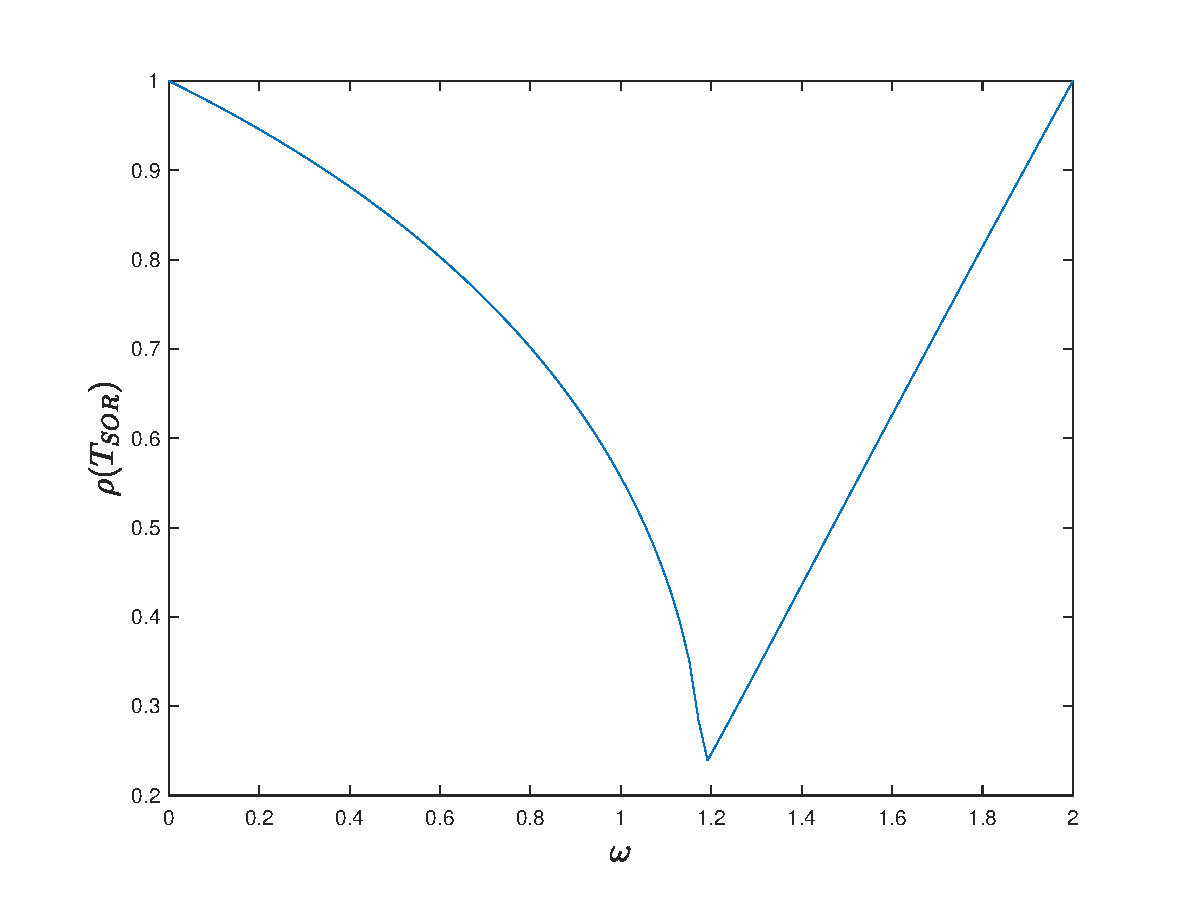
\includegraphics[width=\maxwidth{56.196688409433015em}]{figure_0.eps}
\end{center}

\begin{par}
\begin{flushleft}
The value of $\rho (T_{SOR} )$ is a minimum when $\omega \approx 1.2$ so this is the optimum value.
\end{flushleft}
\end{par}


\vspace{1em}
\label{H_4E3A7150}
\matlabheadingthree{Theorem (optimum relaxation parameters for a positive definite system)}

\begin{par}
\begin{flushleft}
If a system of linear equations of the form $A{x}={b}$ has a positive definite coefficient matrix $A$ with all real eigenvalues then the optimum relaxation parameter for the SOR method can be calculated using
\end{flushleft}
\end{par}

\begin{par}
$$\omega_{opt} =1+{\left(\frac{\rho (T_J )}{1+\sqrt{1-\rho (T_J )^2 }}\right)}^2 ,$$
\end{par}

\begin{par}
\begin{flushleft}
where $T_J$ is the iteration matrix for the Jacobi method.
\end{flushleft}
\end{par}


\vspace{1em}
\label{H_9F7A3728}
\matlabheadingthree{Example 7}

\begin{par}
\begin{flushleft}
Determine the optimum value of the relaxation parameter $\omega$ for the linear system from \hyperref{H_6D573C85}{example 1}. 
\end{flushleft}
\end{par}

\begin{par}
\begin{flushleft}
Checking that $A$ is positive definite
\end{flushleft}
\end{par}

\begin{matlabcode}
A = [ 4, 3, -1 ; 3, 4, -1 ; -1, -1, 4 ];
eig(A)
\end{matlabcode}
\begin{matlaboutput}
ans = 3x1    
    1.0000
    3.4384
    7.5616

\end{matlaboutput}

\begin{par}
\begin{flushleft}
So $\lambda_1 =1$, $\lambda_2 =3.4384$ and $\lambda_3 =7.5616$ which are all real and $A$ is symmetric so $A$ is a positive definite matrix.
\end{flushleft}
\end{par}

\begin{par}
\begin{flushleft}
We saw in \hyperref{H_CB8E1666}{example 6} that $\rho (T_J )=0.7906$, so the optimum value of $\omega$ is
\end{flushleft}
\end{par}

\begin{par}
$$\omega_{opt} =1+{\left(\frac{0.7906}{1+\sqrt{1-0.7906^2 }}\right)}^2 =1.2404.$$
\end{par}


\vspace{1em}
\label{H_493989C7}
\matlabheadingthree{Example 8}

\begin{par}
\begin{flushleft}
Calculate the first iteration of the SOR method using $\omega =1.24$ and the norm of the residual for the system of linear equations from \hyperref{H_6D573C85}{example 1}
\end{flushleft}
\end{par}

\begin{par}
$$\begin{array}{l}
~~~~4x_1 +3x_2 =-2,\\
\,3x_1 +4x_2 -x_3 =-8,\\
\,~~\,\,-x_2 +4x_3 =14.
\end{array}$$
\end{par}

\begin{par}
\begin{flushleft}
The SOR iterations are
\end{flushleft}
\end{par}

\begin{par}
$$\begin{array}{l}
x_1^{(k+1)} =(1-1.24)x_1^{(k)} +\frac{1.24}{4}(-2-3x_2^{(k)} ),\\
x_2^{(k+1)} =(1-1.24)x_2^{(k)} +\frac{1.24}{4}(-8-3x_1^{(k+1)} +x_3^{(k)} ),\\
x_3^{(k+1)} =(1-1.24)x_3^{(k)} +\frac{1.24}{4}(14+x_2^{(k+1)} ).
\end{array}$$
\end{par}

\begin{par}
\begin{flushleft}
Using starting values of ${x}^{(0)} =(0,0,0)^T$ the first iteration is
\end{flushleft}
\end{par}

\begin{par}
$$\begin{array}{l}
x_1^{(k+1)} =(1-1.24)(0)+\frac{1.24}{4}(-2-3(0))=-0.62,\\
x_2^{(k+1)} =(1-1.24)(0)+\frac{1.24}{4}(-8-3(-0.62)+0)=-1.9034,\\
x_3^{(k+1)} =(1-1.24)(0)+\frac{1.24}{4}(14-1.9034)=3.74995.
\end{array}$$
\end{par}

\begin{par}
\begin{flushleft}
Calculate the residual
\end{flushleft}
\end{par}

\begin{par}
$${r}^{(1)} ={b}-A{x}^{(1)} =\left(\begin{array}{c}
-2\\
-8\\
14
\end{array}\right)-\left(\begin{array}{ccc}
4 & 3 & 0\\
3 & 4 & -1\\
0 & -1 & 4
\end{array}\right)\left(\begin{array}{c}
-0.62\\
-1.9034\\
3.74995
\end{array}\right)=\left(\begin{array}{c}
6.1902\\
5.2235\\
-2.9032
\end{array}\right)$$
\end{par}

\begin{par}
\begin{flushleft}
and the norm of the residual is $|{r}^{(1)} |=\sqrt{6.1902^2 +5.2235^2 +(-2.9032)^2 }=8.60421.$
\end{flushleft}
\end{par}


\vspace{1em}
\label{H_D8882FA8}
\matlabheadingthree{Example 9}


\vspace{1em}
\begin{matlabcode}
% Define linear system
A = [ 4, 3, 0 ; 3, 4, -1 ; 0, -1, 4 ];
b = [ -2 ; -8 ; 14 ];

% Solve linear system using the Jacobi method
x = sor(A, b, 1.24, 100, 1e-4);

% Ouput solution table
N = length(b);
table = '  k      ';
for i = 1 : N
    table = [ table, sprintf('x_%1i       ', i)];
end
table = [ table, sprintf('|r|\n%s\n', repmat('-', 1, 4 + (N + 1) * 10)) ];
for k = 1 : size(x, 1)
    table = [ table, sprintf('%4i', k - 1) ];
    table = [ table, sprintf('%10.5f', x(k, :)) ];
    table = [ table, sprintf('%10.5f\n', norm(b - A * x(k,:)')) ];
end
fprintf(table)
\end{matlabcode}
\begin{matlaboutput}
  k      x_1       x_2       x_3       |r|
--------------------------------------------
   0   0.00000   0.00000   0.00000  16.24808
   1  -0.62000  -1.90340   3.74995   8.60421
   2   1.29896  -2.06874   2.79870   1.48306
   3   0.99217  -2.03863   3.03634   0.31850
   4   1.03780  -2.01462   2.98675   0.13283
   5   1.00452  -2.00481   3.00169   0.01419
   6   1.00338  -2.00147   2.99914   0.01066
   7   1.00055  -2.00043   3.00007   0.00118
   8   1.00027  -2.00012   2.99994   0.00080
   9   1.00005  -2.00003   3.00000   0.00011
  10   1.00002  -2.00001   3.00000   0.00006
\end{matlaboutput}

\begin{par}
\begin{flushleft}
Note that the SOR method took 10 iterations to achieve convergence to $tol=10^{-4}$ whereas the Gauss-Seidel and Jacobi methods took 20 and 50 iterations respectively to achieve the same accuracy.
\end{flushleft}
\end{par}



\vspace{1em}
\label{H_EB3CCAC9}
\matlabheading{Summary}

\begin{itemize}
\setlength{\itemsep}{-1ex}
   \item{\begin{flushleft} \hyperref{H_52186026}{Indirect methods} use an iterative approach to improve an estimate of the solution to a system of linear equations. The methods are iterated until the estimates have achieved the required accuracy. \end{flushleft}}
   \item{\begin{flushleft} The \hyperref{H_55926E44}{Jacobi method} is uses information from the previous iteration only to update the estimates. \end{flushleft}}
   \item{\begin{flushleft} The \hyperref{H_CAC75FFA}{Gauss-Seidel method} uses values of estimates already calculated in a given iteration to update the estimates. This means that the Gauss-Seidel method will converge to a solution faster than the Jacobi method.  \end{flushleft}}
   \item{\begin{flushleft} An indirect method will converge to the exact solution if the value of the \hyperref{C70E30F2}{spectral radius} (the largest absolute eigenvalue) of the iteration matrix for a linear system is less than 1.  \end{flushleft}}
   \item{\begin{flushleft} The smaller the value of the spectral radius, the faster the method will converge to the exact solution. \end{flushleft}}
   \item{\begin{flushleft} The \hyperref{H_0296912E}{SOR method} uses a relacation parameter to adjust how much estimates will change over a single iteration. The value of the relaxation parameter is chosen to minimise the spectral radius.  \end{flushleft}}
\end{itemize}



\vspace{1em}
\label{H_354E4A4B}
\matlabheading{Exercises}


\vspace{1em}
\begin{par}
\begin{flushleft}
1.    Calculate the first 2 iterations of the Jacobi method for solving the system of linear equations below. Use starting values of $x_i^{(0)} =0$ and work to 4 decimal places.
\end{flushleft}
\end{par}

\begin{par}
$$\begin{array}{l}
4x_1 +x_2 -x_3 +x_4 =14,\\
x_1 +4x_2 -x_3 -x_4 =10,\\
-x_1 -x_2 +5x_3 +x_4 =-15,\\
x_1 -x_2 +x_3 +3x_4 =3.
\end{array}$$
\end{par}

\begin{par}
\begin{flushleft}
2.     Repeat question 1 using the Gauss-Seidel method.
\end{flushleft}
\end{par}

\begin{par}
\begin{flushleft}
3.     Repeat question 1 using the SOR method using the optimum value for the relaxation parmeter.
\end{flushleft}
\end{par}

\begin{par}
\begin{flushleft}
4.     Which method would you expect to converge to the solution with the fewest iterations? What quantitative evidence do you have to support your conclusion?
\end{flushleft}
\end{par}

\begin{par}
\begin{flushleft}
5.     Write a MATLAB program to calculate the solution to questions 1 - 3 using $tol=10^{-5}$.
\end{flushleft}
\end{par}

\begin{par}
\begin{flushleft}
6.    A linear system has the following coefficient matrix. What is the largest value that $\alpha$ can be in order for the Jacobi method to be convergent?
\end{flushleft}
\end{par}

\begin{par}
$$A=\left(\begin{array}{cc}
2 & 1\\
\alpha  & 2
\end{array}\right)$$
\end{par}

\begin{par}
\begin{flushleft}
7.     A linear system has the following coefficient matrix. Is the Jacobi method convergent for this system? If not, can the system be altered so that the Jacobi method is convergent?
\end{flushleft}
\end{par}

\begin{par}
$$A=\left(\begin{array}{ccc}
1 & 3 & 1\\
2 & 1 & 0\\
1 & 1 & 4
\end{array}\right)$$
\end{par}


\label{H_712F20E0}
\vspace{1em}

\label{H_44DDF0D5}
\matlabheading{Functions}

\begin{par}
\begin{flushleft}
The various functions used in this page are defined in this section.
\end{flushleft}
\end{par}

\label{H_81F8E1E6}
\matlabheadingthree{Jacobi method}

\begin{par}
\hfill \break
\end{par}

\begin{matlabcode}
function x = jacobi(A, b, maxiter, tol)

% Calculates the solution to the system of linear equations Ax = b using
% the Jacobi method

% Initialise solution array
N = length(b);
x = zeros(maxiter + 1, N);

% Iteration loop
for k = 1 : maxiter
    
    % Calculate Jacobi method
    for i = 1 : N
        
        % Calculate sum
        for j = 1 : N
            if i ~= j
                x(k+1, i) = x(k+1, i) + A(i, j) * x(k, j);
            end
        end
        
        % Calculate new estimate of x(i)
        x(k+1, i) = (b(i) - x(k+1, i)) / A(i, i);
    end
    
    % Calculate norm of the residual
    r = norm(b - A * x(k+1, :)');
    
    % Check for convergence
    if r < tol
        break
    end
    
end

% Trim x array
x(k+2:end, :) = [];

end
\end{matlabcode}

\label{H_FECB29ED}
\vspace{1em}

\label{H_16F3405C}
\matlabheadingthree{Gauss-Seidel method}

\begin{par}
\hfill \break
\end{par}

\begin{matlabcode}
function x = gauss_seidel(A, b, maxiter, tol)

% Calculates the solution to the system of linear equations Ax = b using
% the Gauss-Seidel method

% Initialise solution array
N = length(b);
x = zeros(maxiter + 1, N);

% Iteration loop
for k = 1 : maxiter
    
    % Calculate Gauss-Seidel method
    for i = 1 : N
        
        % Calculate sum
        for j = 1 : N
            if j < i
                x(k+1, i) = x(k+1, i) + A(i, j) * x(k+1, j);
            elseif j > i
                x(k+1, i) = x(k+1, i) + A(i, j) * x(k, j);
            end
        end
        
        % Calculate new estimate of x(i)
        x(k+1, i) = (b(i) - x(k+1, i)) / A(i, i);
    end
    
    % Calculate norm of the residual
    r = norm(b - A * x(k+1, :)');
    
    % Check for convergence
    if r < tol
        break
    end
    
end

% Trim x array
x(k+2:end, :) = [];

end
\end{matlabcode}

\label{H_02474416}
\vspace{1em}

\label{H_4725A5A1}
\matlabheadingthree{SOR method}

\begin{par}
\hfill \break
\end{par}

\begin{matlabcode}
function x = sor(A, b, omega, maxiter, tol)

% Calculates the solution to the system of linear equations Ax = b using
% the SOR method

% Initialise solution array
N = length(b);
x = zeros(maxiter + 1, N);

% Iteration loop
for k = 1 : maxiter
    
    % Calculate Jacobi method
    for i = 1 : N
        
        % Calculate sum
        for j = 1 : N
            if j < i
                x(k+1, i) = x(k+1, i) + A(i, j) * x(k+1, j);
            elseif j > i
                x(k+1, i) = x(k+1, i) + A(i, j) * x(k, j);
            end
        end
        
        % Calculate new estimate of x(i)
        x(k+1, i) = (1 - omega) * x(k, i) + omega * (b(i) - x(k+1, i)) / A(i, i);
    end
    
    % Calculate norm of the residual
    r = norm(b - A * x(k+1, :)');
    
    % Check for convergence
    if r < tol
        break
    end
    
end

% Trim x array
x(k+2:end, :) = [];

end
\end{matlabcode}

\end{document}
